\chapter{Architettura}
\section{Introduzione}

\section{Diagrammi delle classi}
\begin{figure}[ht]
	\centering
	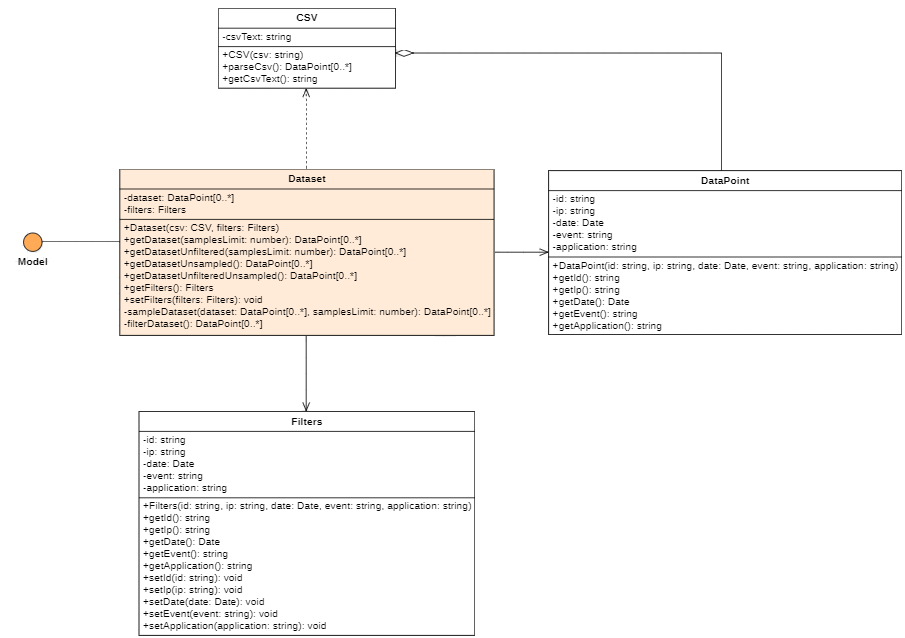
\includegraphics[width=\textwidth]{Model.png}
	\caption{Diagramma Model}
  \end{figure}
La funzione del modello è separare la logica dei dati dall'interfaccia.\\
Il diagramma delle classi del Model è costituito dall'interfaccia \textbf{\texttt{Model}} e dalle classi concrete \texttt{Dataset}, \texttt{Filters}, \texttt{DataPoint} e \texttt{CSV}.
Nel dettaglio la funzione delle varie componenti del model è:
\begin{itemize}
	\item \texttt{Filters}: è la classe che permette la gestione dei filtri applicati al grafico. Presenta dei metodi "get" e "set" per ogni campo dati presente, che permettono di recuperare oppure salvare i filtri applicati al grafico.
	\item \texttt{DataPoint}: è la classe che permette di salvare al suo interno le informazioni ottenute dalle tuple del file ".csv";
	\item \texttt{CSV}: è la classe che permette di salvare le informazioni presenti nel file ".csv" caricato, con il formato di array di \texttt{DataPoint};
	\item \texttt{Dataset}: è la classe più importante del Modello in quanto, oltre a salvare al suo interno tutti i filtri applicati ai grafici, salva e gestisce tutte le informazioni lette dal file ".csv" caricato.\\ La classe \texttt{Dataset} mette a disposizione differenti metodi che permettono di ottenere e salvare i filtri, salvare le informazioni dei file ".csv" e recuperare tali informazioni con delle varianti (come privarle o meno di filtri e campionature).
\end{itemize}
\subsection{View}


\begin{figure}[ht]
	\centering
	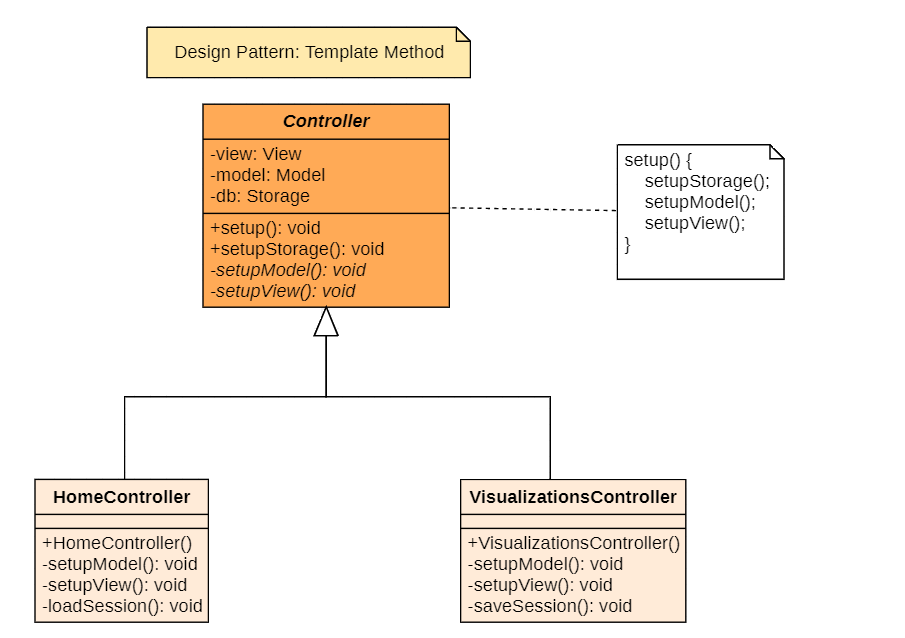
\includegraphics[width=\textwidth]{Controller.png}
	\caption{Diagramma Controller}
  \end{figure}
Il controller agisce da intermediario tra vista e modello. Ha la funzione di soddisfare le richieste poste da parte dell'utente modificando le altre due componenti.\\
Possiamo notare la presenza di una classe astratta chiamata \textbf{\texttt{Controller}} che definisce i valori e i metodi che le istanze dovranno presentare.\\
La scelta di usare due controller nell'applicazione è stata fatta per riuscire a gestire le pagine, con differenti funzionalità, in modo semplice e modulare permettendo una più semplice estendibilità e manutenibilità.\\
\textbf{HomeController} e \textbf{VisualizationsController} sono gli oggetti istanziabili con superclasse \textbf{\texttt{Controller}} e sono utilizzati nel seguente modo: 
\begin{itemize}
	\item \textbf{HomeController}: Ha la funzione di gestire l'interazione Model-View nella scheda iniziale. Caratteristica di questa classe è la presenza del metodo privato \texttt{loadSession()} che permette il caricamento di un dataset oppure di una sessione precedentemente salvata.
	\item \textbf{VisualizationsController}: Ha la funzione di gestire l'interazione Model-View nella scheda in cui vengono visualizzati i grafici con i vari filtri. La caratteristica di questa classe è la presenza del metodo privato \texttt{saveSession()} che permette di salvare la sessione in corso con il grafico visualizzato e i filtri applicati.
\end{itemize}
Entrambe le classi precedentemente citate hanno il metodo comune \texttt{setup()} che permette l'inizializzazione della classe andando a chiamre altri tre metodi: \texttt{setupStorage()} che genera l'istanza della classe \texttt{IndexedDB}, \texttt{setupModel()} che istanzia il Modello e \texttt{setupView()} che crea la View. Completato il processo di inizializzazione l'applicazione sarà pronta a rispondere alle interazioni con l'utente.

\section{Diagrammi di sequenza}
\subsection{Caricamento dataset}
\begin{figure}[H]
	\centering
	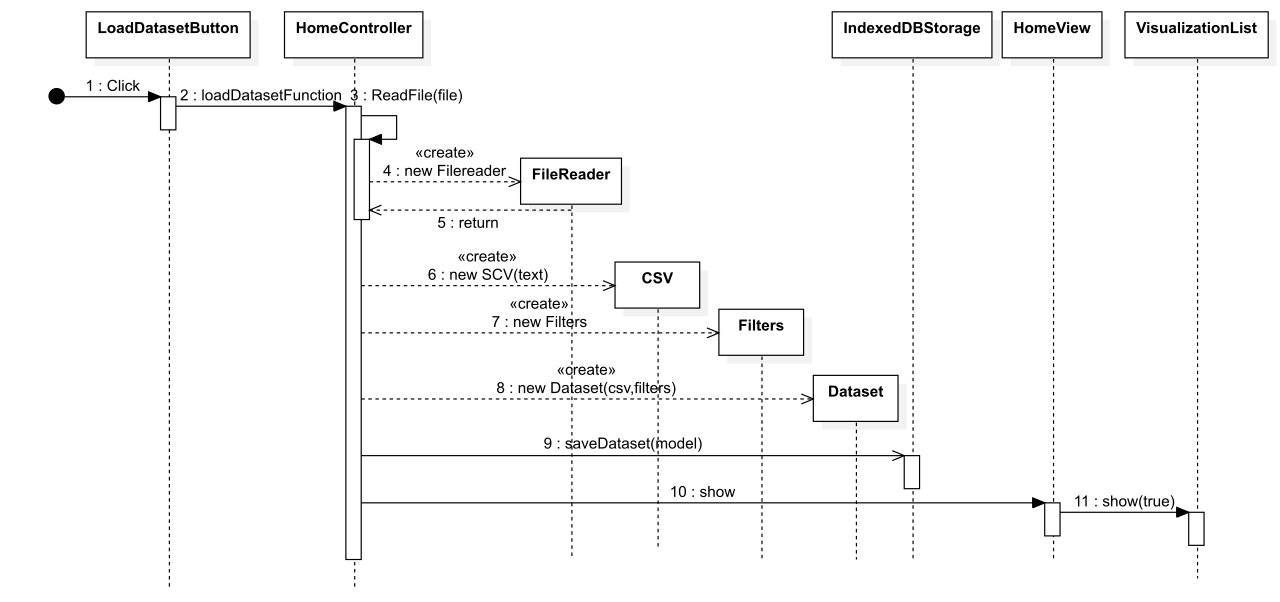
\includegraphics[width=\textwidth]{SequenceDiagramLoadDatasetButton.jpg}
	\caption{Diagramma Strategy pattern}
  \end{figure}
  La sequenza di azioni che portano al caricamento del dataset e alla conseguente visualizzazione dei vari grafici disponibili sono innescate dal "click" effettuato dall'utente sull'oggetto \texttt{LoadDatasetButton}.\\
Una volta cliccato \texttt{LoadDatasetButton} emetterà un segnale recepito, tramite gli EventListner, dalla classe \texttt{HomeController} che eseguirà la funzione \texttt{loadDatasetFunction()}. Tale funzione chiamerà a sua volta un'altra funzione appartenente alla classe \texttt{HomeController} chiamata \texttt{ReadFile()}.
\texttt{ReadFile()} andrà semplicemente a creare un oggetto \texttt{FileReader} a cui verrà fatto leggere, sotto forma di testo, il dataset passato dall'utente. \\
Una volta terminata l'esecuzione della funzione \texttt{ReadFile()} continuerà l'esecuzione della funzione \texttt{LoadDatasetButton} andando a creare tre oggetti: 
\texttt{CSV} a cui verrà passato come parametro attuale ciò che è stato letto da \texttt{FileReader}, \texttt{Filters} e \texttt{Dataset} a cui vengono passati come parametri attuali gli oggetti precedentemente creati \texttt{CSV} e \texttt{FileReader}.
Il passo successivo compiuto dalla funzione è chiamare il metodo \texttt{saveDataset()} dell'oggetto \texttt{IndexedDBStorage} a cui viene passato l'oggetto crato precedentemente \texttt{Dataset} con lo scopo di salvarlo nel database esterno all'applicazione.
Come ultimo passo viene chiamata la funzione \texttt{show()} dell'oggetto \texttt{VisualizationList} che permetterà la visualizzazione delle configurazioni dei grafici disponibili all'interno della HomePage.

\subsection{Diagramma di sequenza del caricamento del dataset}

\section{Design pattern utilizzati}
\subsection{Strategy}
\begin{figure}[H]
	\centering
	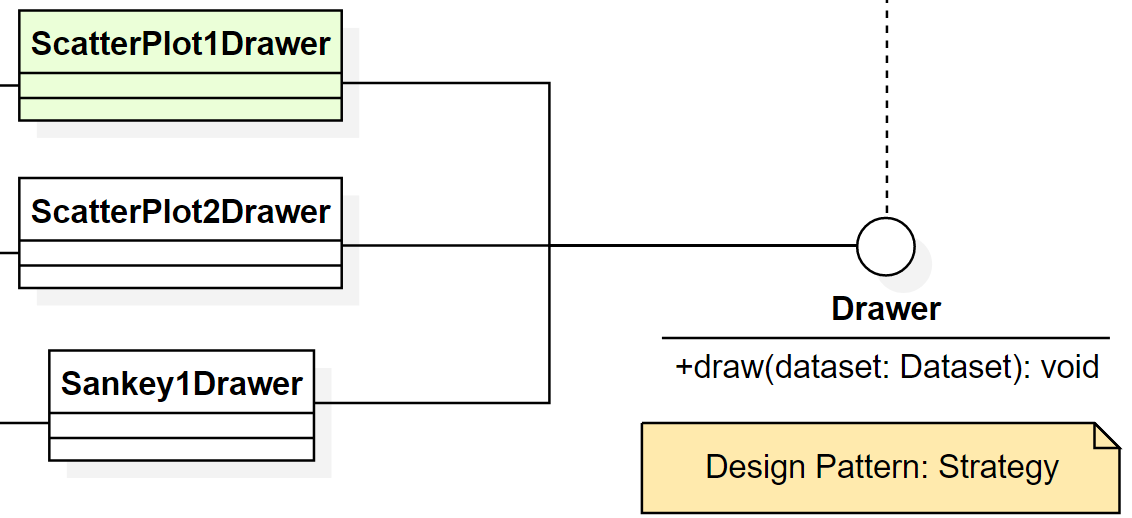
\includegraphics[width=\textwidth]{StrategyPattern.png}
	\caption{Diagramma Strategy pattern}
  \end{figure}
Il nostro gruppo ha scelto di utilizzare il pattern \textit{Strategy} per la generazione dei grafici in quanto ci serviva un algoritmo il cui fine era il medesimo, ma che sfruttasse passi differenti per la rappresentazione delle differenti viste.\\
Come è possibile notare dall'immagine lo \texttt{Strategy} presenta un'interfaccia chiamata \texttt{Drawer} la quale dichiara un metodo \texttt{draw(dataset:Dataset)} che sarà definito in maniera differente dalle classi che implmenteranno l'interfaccia, in questo modo sarà possibile la generazione di grafici differenti.\\
Dall'immagine possiamo notare solamente tre differenti classi che implmentano "Drawer" che sono "ScatterPlot1", "ScatterPlot2" e "Sankey1Diagram"; questo è stato fatto per una questione di semplicità espositiva, in realtà ogni configurazione dei vari grafici avrà la propria classe specifica per la rappresentazione del dataset. \\

\subsection{Template method}

